\documentclass[11pt]{article}
\usepackage{amsmath}
\usepackage{graphicx}
\usepackage{hyperref}
\usepackage[utf8]{inputenc}
\usepackage[spanish]{babel}
\usepackage[margin=2cm]{geometry}
\usepackage{amsfonts}
\usepackage{listings}
\usepackage[T1]{fontenc}
\usepackage{float}
\usepackage{subfig}

\title{Práctica 1 Minería de Texto - Minería de Medios Sociales.}
\author{Curso: 2018/2019. Néstor Rodríguez Vico. DNI: 75573052C - \href{mailto:nrv23@correo.ugr.es}{nrv23@correo.ugr.es}}
\date{\today}


\lstdefinestyle{bash_style}{
	language=bash,
	frame=single,
	xleftmargin=.25in,
	upquote = true,
	basicstyle=\scriptsize,
	breakatwhitespace=false,         
	breaklines=true,                 
	captionpos=b,                    
	keepspaces=true,                 
	numbers=left,                    
	numbersep=5pt,                  
	showspaces=false,                
	showstringspaces=false,
	showtabs=false,                  
	tabsize=2
}

\lstset{style=bash_style}

\begin{document}
\maketitle

\setlength{\belowdisplayskip}{5pt} 
\setlength{\belowdisplayshortskip}{5pt}
\setlength{\abovedisplayskip}{5pt} 
\setlength{\abovedisplayshortskip}{5pt}

\section{Introducción.}

Los datos usados para realizar esta práctica han sido obtenidos tras realizar la búsqueda \textit{Documents classification} en \textit{Google}. Dicha búsqueda lleva a muchas competiciones de \textit{Kaggle}. Muchas de ellas son privadas (se necesita una invitación para poder descargar los dataset) pero en una de ellas (\href{https://www.kaggle.com/yufengdev/bbc-fulltext-and-category}{https://www.kaggle.com/yufengdev/bbc-fulltext-and-category}) se puede descargar un conjunto de datos proveniente de la página de la \href{http://mlg.ucd.ie/datasets/bbc.html}{BBC} (\href{http://mlg.ucd.ie/datasets/bbc.html}{http://mlg.ucd.ie/datasets/bbc.html}). Esta colección consiste en \textit{2225} documentos provenientes del sitio web de noticias de la  \textit{BBC}, correspondientes a historias de cinco áreas temáticas de 2004-2005. Dichas áreas son: negocios, entretenimiento, política, deporte, tecnología. Dicho conjunto de datos cuenta con \textit{2225} documentos.

\section{Workflow.}

El \textit{workflow} desarrollado es el siguiente:

\begin{figure}[H]
	\centering
	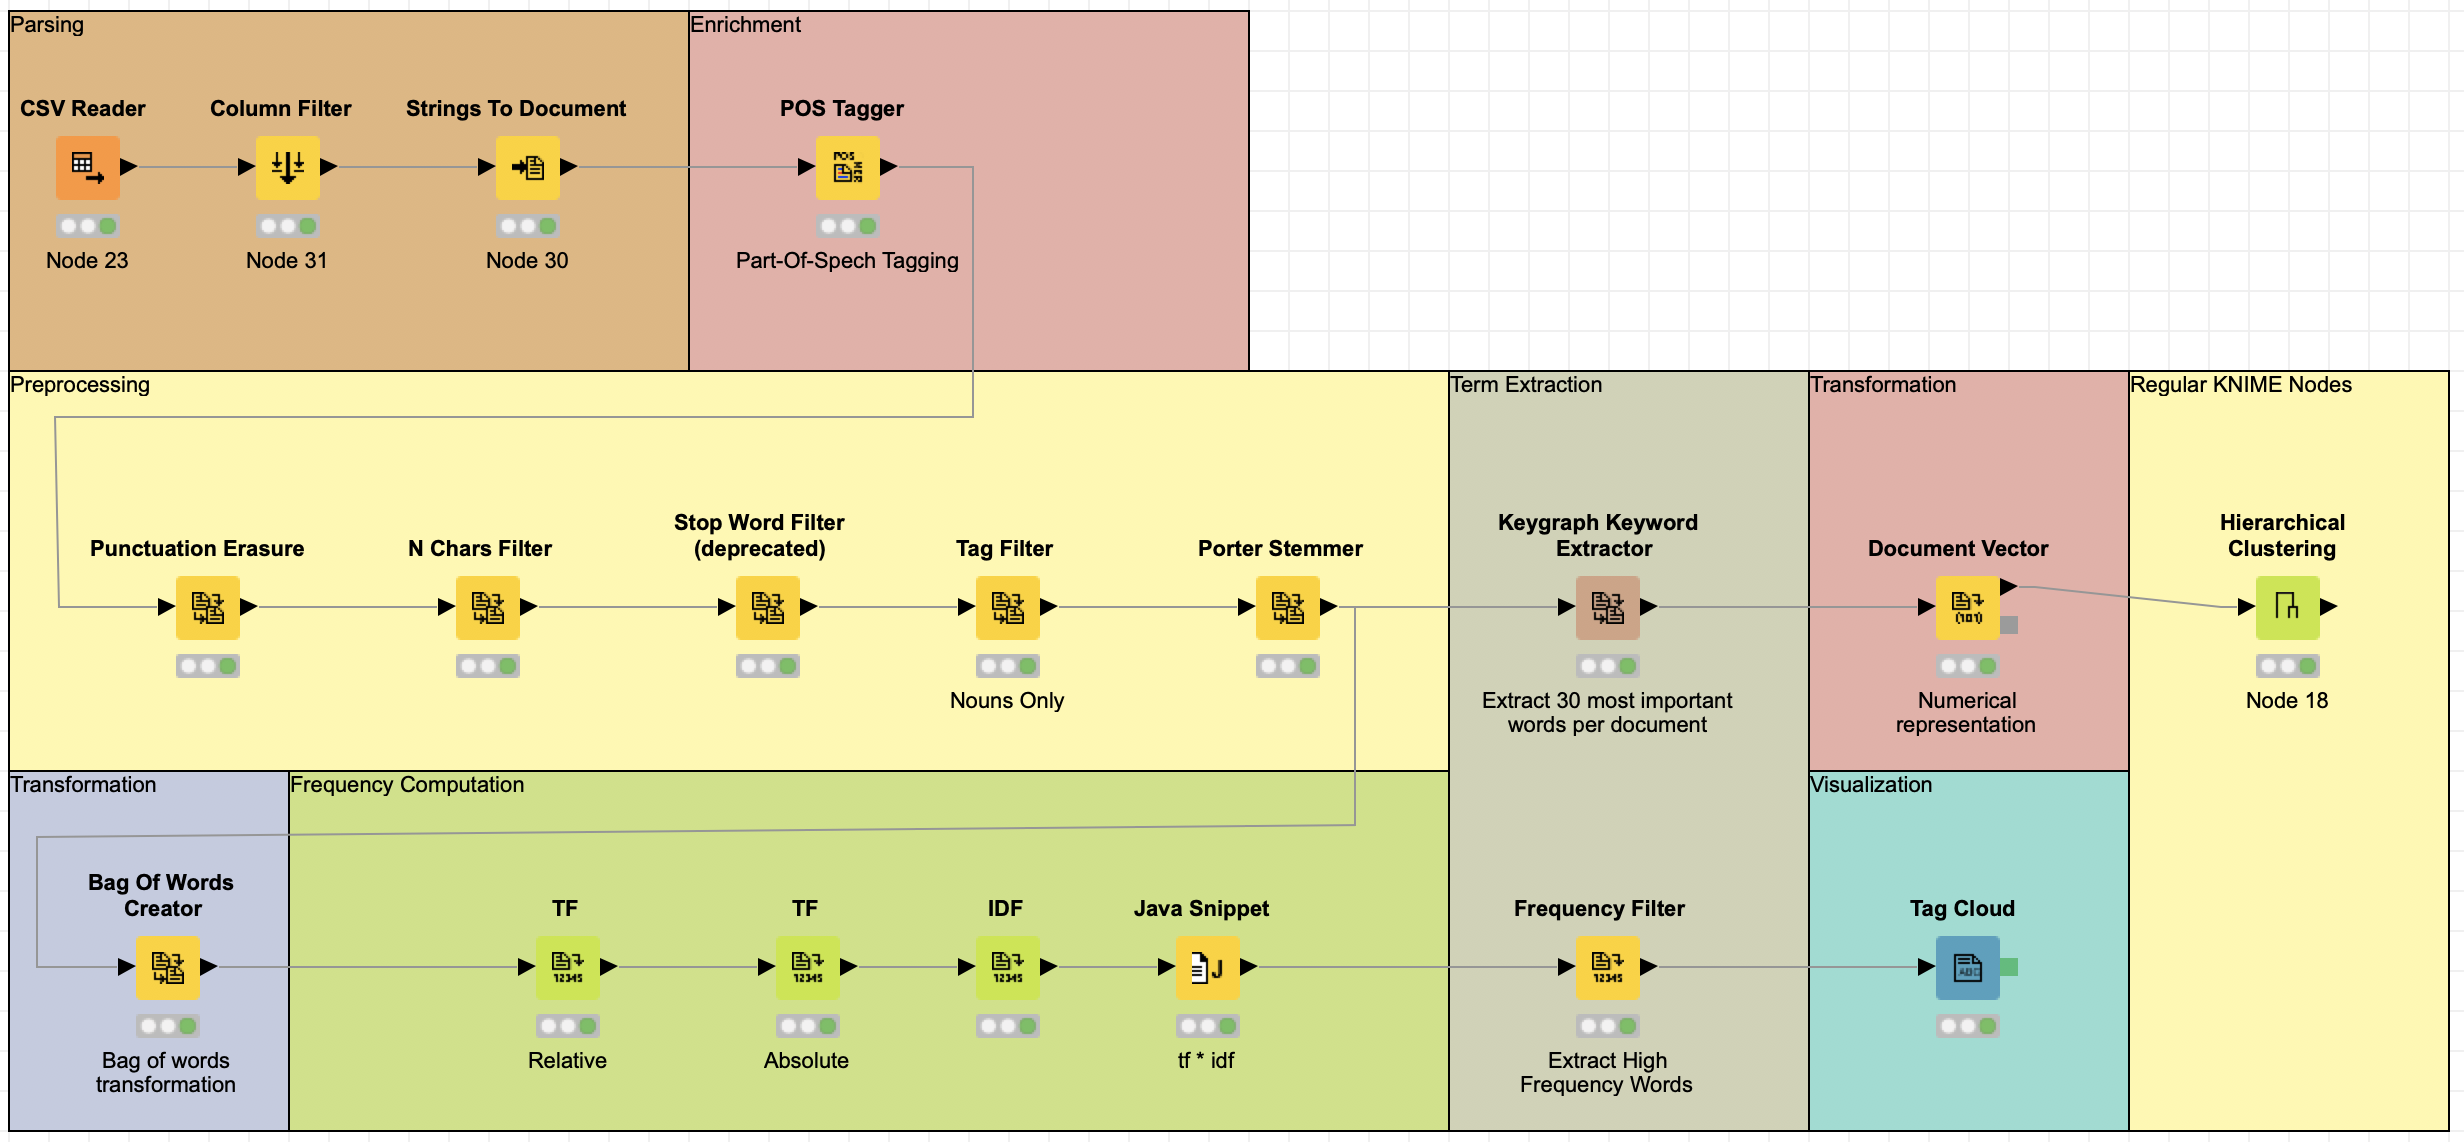
\includegraphics[width=\linewidth]{images/workflow.png}
\end{figure}

Se ha cogido el \textit{workflow} proporcionado y se han hecho los siguientes cambios:

\begin{itemize}
	\item Se ha cambiado como se obtiene la colección de documentos. En este caso se ha empleado un lector de \textit{CSV}. Una vez leidos los documentos, mandamos la información a un nodo que flitra las columnas para quedarnos solo con la columna que contiene la información del documento en sí.
	\item Una vez tenemos los datos limpios, convertimos el texto que representa el documento a una variable de tipo \textit{Document}, que es el tipo usado por \textit{KNIME} para representar un documento.
	\item En la sección de enriquecimiento he quitado el nodo \textit{Abner Tagger} ya que es un preprocesamiento específico para el problema original propuesto y no aplica en el problema presentado en esta memoria.
\end{itemize}

El resto del \textit{workflow} se mantiene de la misma forma:
\begin{itemize}
	\item Eliminamos los signos de puntuación con el nodo \textit{Punctuation Erasure}.
	\item Eliminamos las palabas con un tamaño menor que \textit{N}, en nuestro caso $3$, con el nodo \textit{N Chars Filter}.
	\item Eliminamos las palabras vacías con el nodo \textit{Stop Word Filter}. En nuestro caso, hemos usado la lista de \textit{stopwords} proveída por \textit{KNIME} para el idioma del problema, \textit{inglés}.
	\item Eliminamos las palabras que tienen una etiqueta asociada, es decir, son palabras de una categoría concreta con el nodo \textit{Tag Filter}. Por ejemplo, eliminamos los pronombres, ya que no nos aportan nada.
	\item Finalmente, aplicamos el algoritmos de \textit{Porter} con el nodo \textit{Porter Stemmer} para quedarnos con la raíz de las palabras.
\end{itemize}

Tras ejecutar el primer y segundo nodo ya tenemos el texto de los documentos cargados. Para ver el contenido de dicho nodo podemos pinchar en el segundo nodo y elegir la última opción del menú para mostrar los datos, la opción \textit{Filtered table}. El resultado es el siguiente:

\begin{figure}[H]
	\centering
	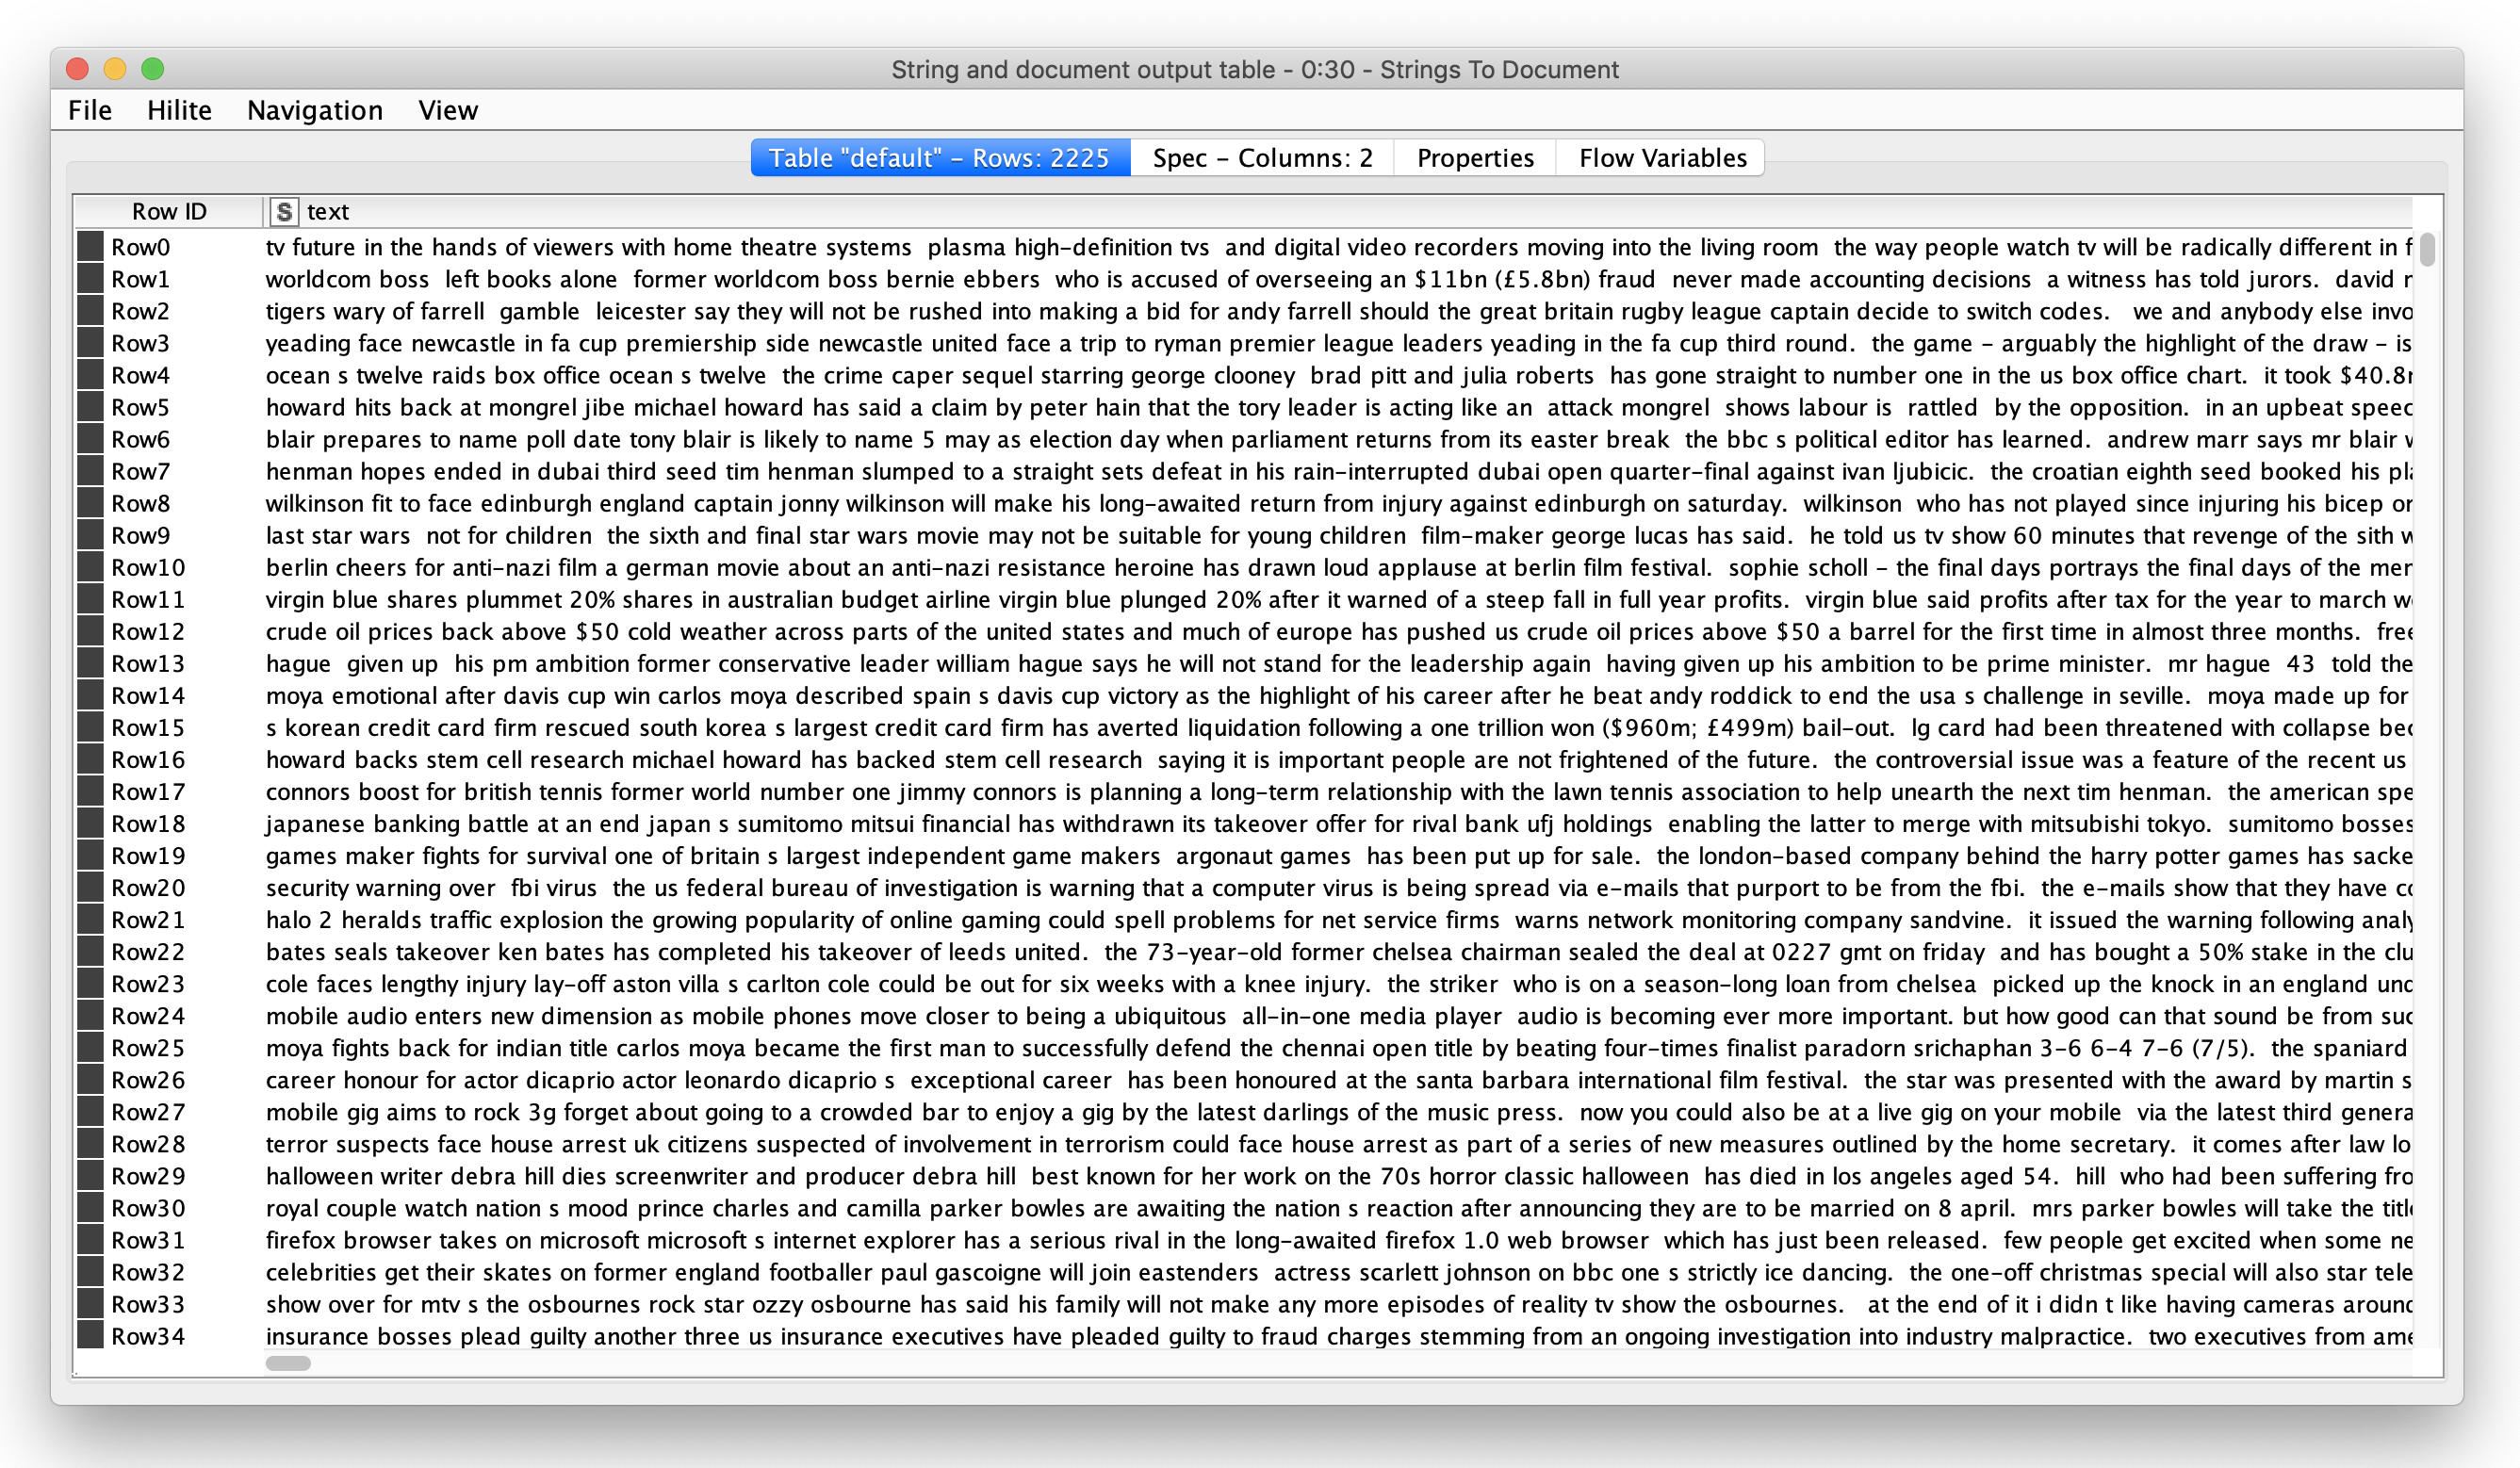
\includegraphics[width=0.9\linewidth]{images/raw.png}
\end{figure}

Tras ejecutar todos los nodoes de la sección \textit{Parsing}, de la sección \textit{Enrichment} y de la sección \textit{Preprocessing} tenemos un conjunto de datos ya preprocesado y limpio. Podemos ver como ha quedado dicho conjunto si hacemos click derecho en el nodo \textit{Porter Stemmer} y seleccionamos la última opción del menú, la opción \textit{Preprocessed documents}. El resultado es el siguiente:

\begin{figure}[H]
	\centering
	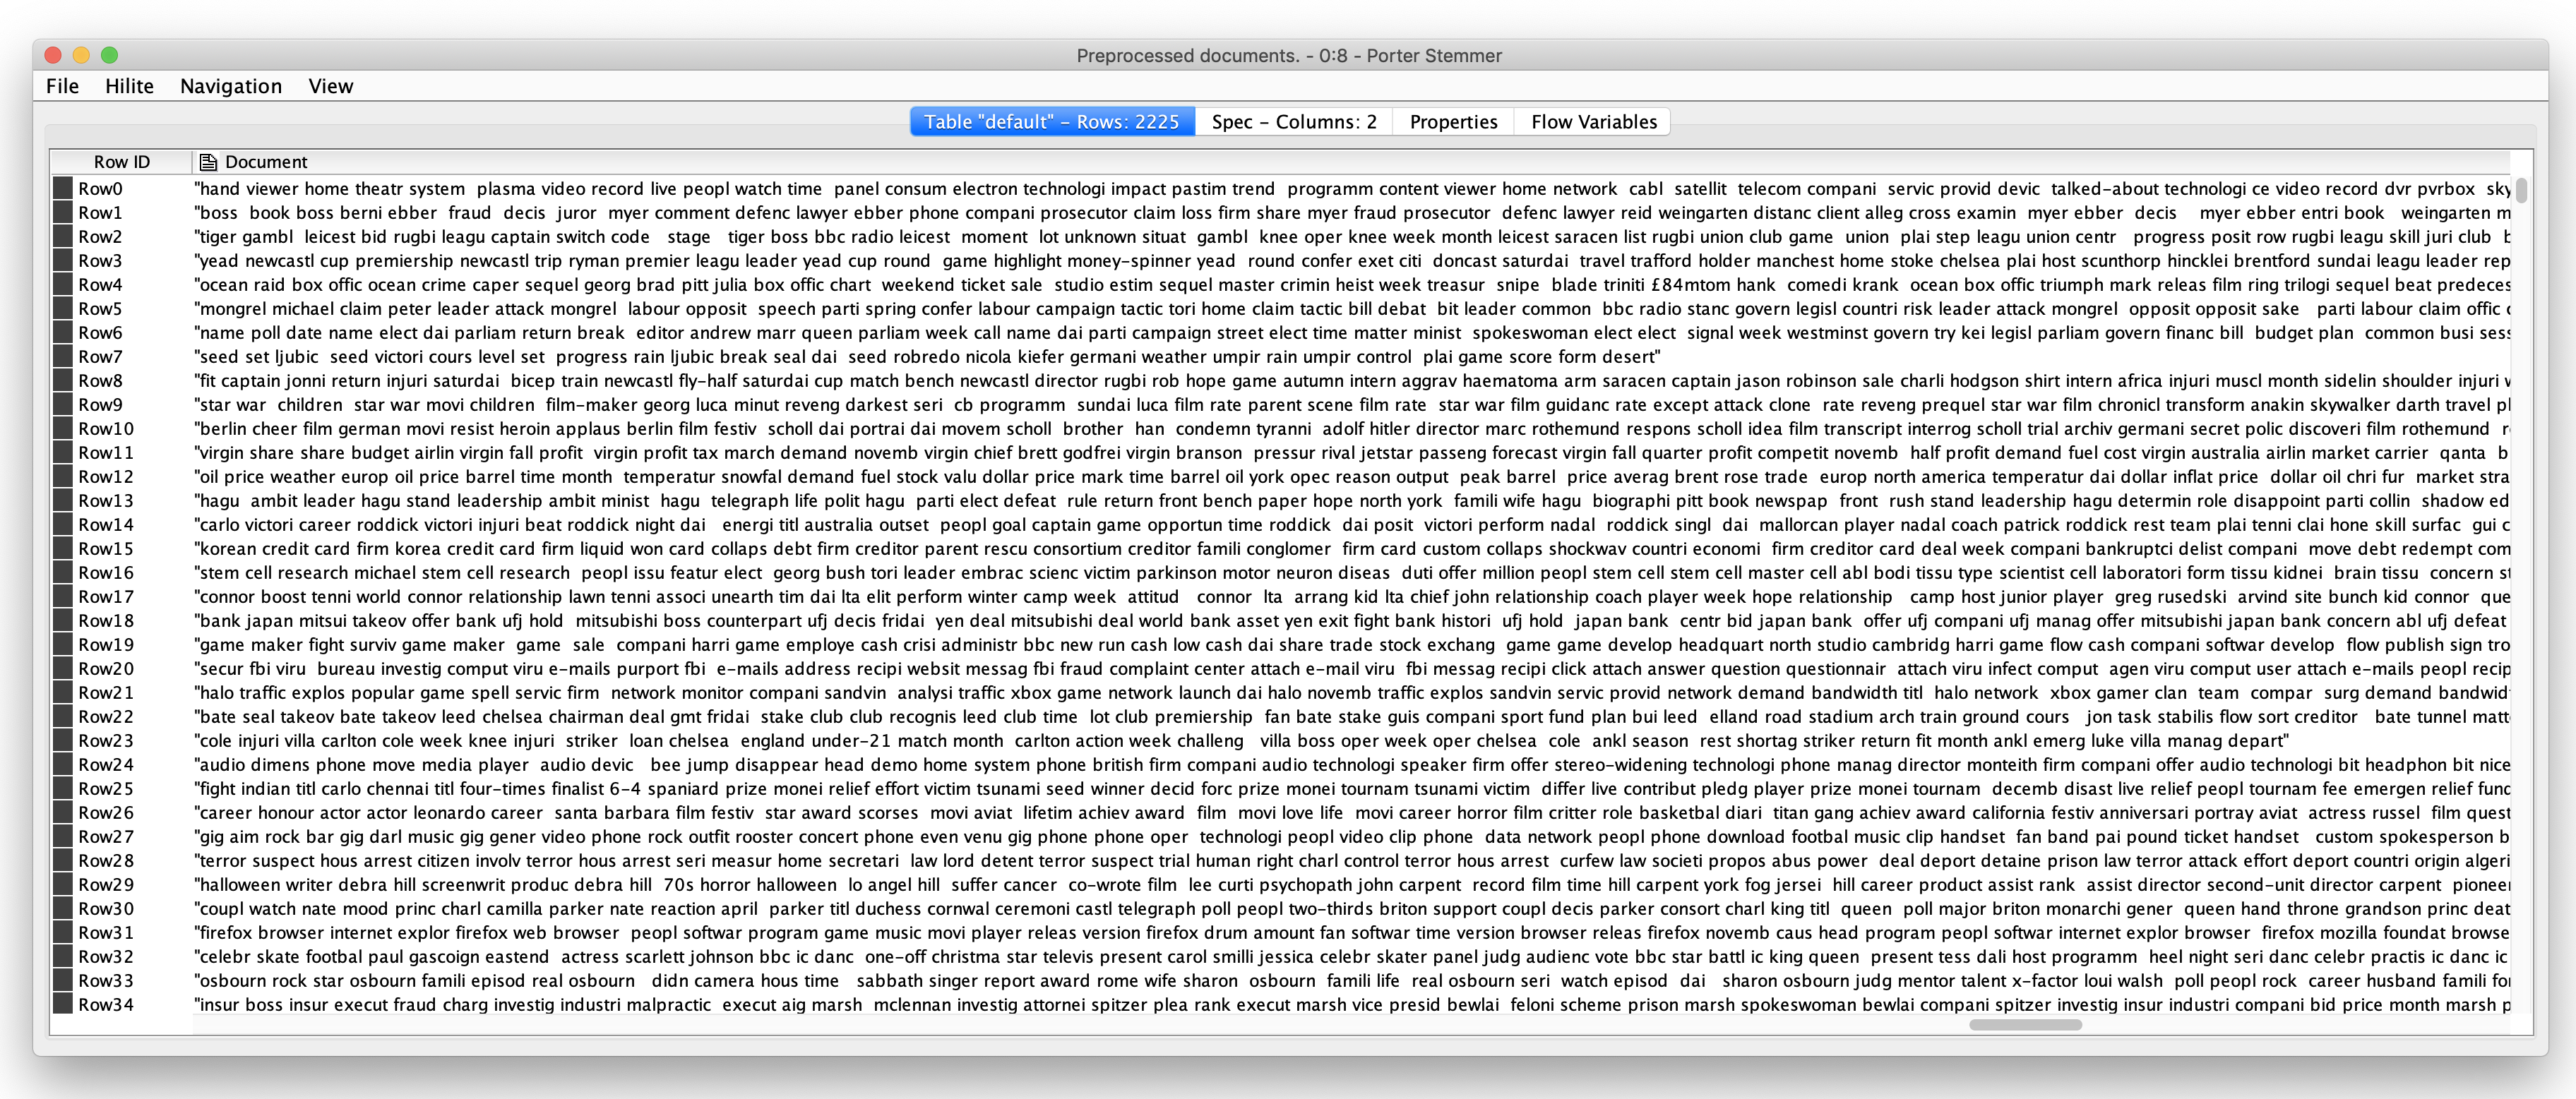
\includegraphics[width=0.9\linewidth]{images/preprocessed.png}
\end{figure}

Si comparamos los resultados podemos ver las diferencias que hemos aplicado en los nodos. Por ejemplo, podemos ver como el documento representado en la línea identificada por \textit{Row3} ha desaparecido el punto que hay. También podemos observar como han desaparecido las palabras con una longitud menor que \textit{3}. Aunque los cambios más notables son cómo hemos sido capaces de eliminar las \textit{stopwords}, eliminar ciertas palabras que tienen una etiqueta asociada y el quedarnos con la raiz de las palabras. Estas tres técnicas nos permiten limpiar los documentos de palabras vacías de contenido (como pueden ser las \textit{stopwords} o las palaras que tienen una etiqueta asociada y no nos interesan, como pueden ser los pronombres). Finalmente, nos hemos quedado con la raiz de las palabras, lo cual permite generalizar que texto es usado para entrenar nuestro modelo. Esta idea permite reconocer la palabra \textit{comer} y la palabra \textit{comes} como la misma, ya que su raiz es la misma. \\

Finalmente, usamos un nodo \textit{Tag Cloud}, el cual genera una nube de etiquetas. Una nube de etiquetas es una representación de palabras que indica la importancia de las palabras de una forma visual, jugando con el tamaño y la transparencia del texto mostrado. En mi caso, las palabras más relevantes son \textit{tottenham}, \textit{librari} y \textit{godzilla}, tal y como podemos ver en la nube de etiquetas generada por el \textit{workflow}:

\begin{figure}[H]
	\centering
	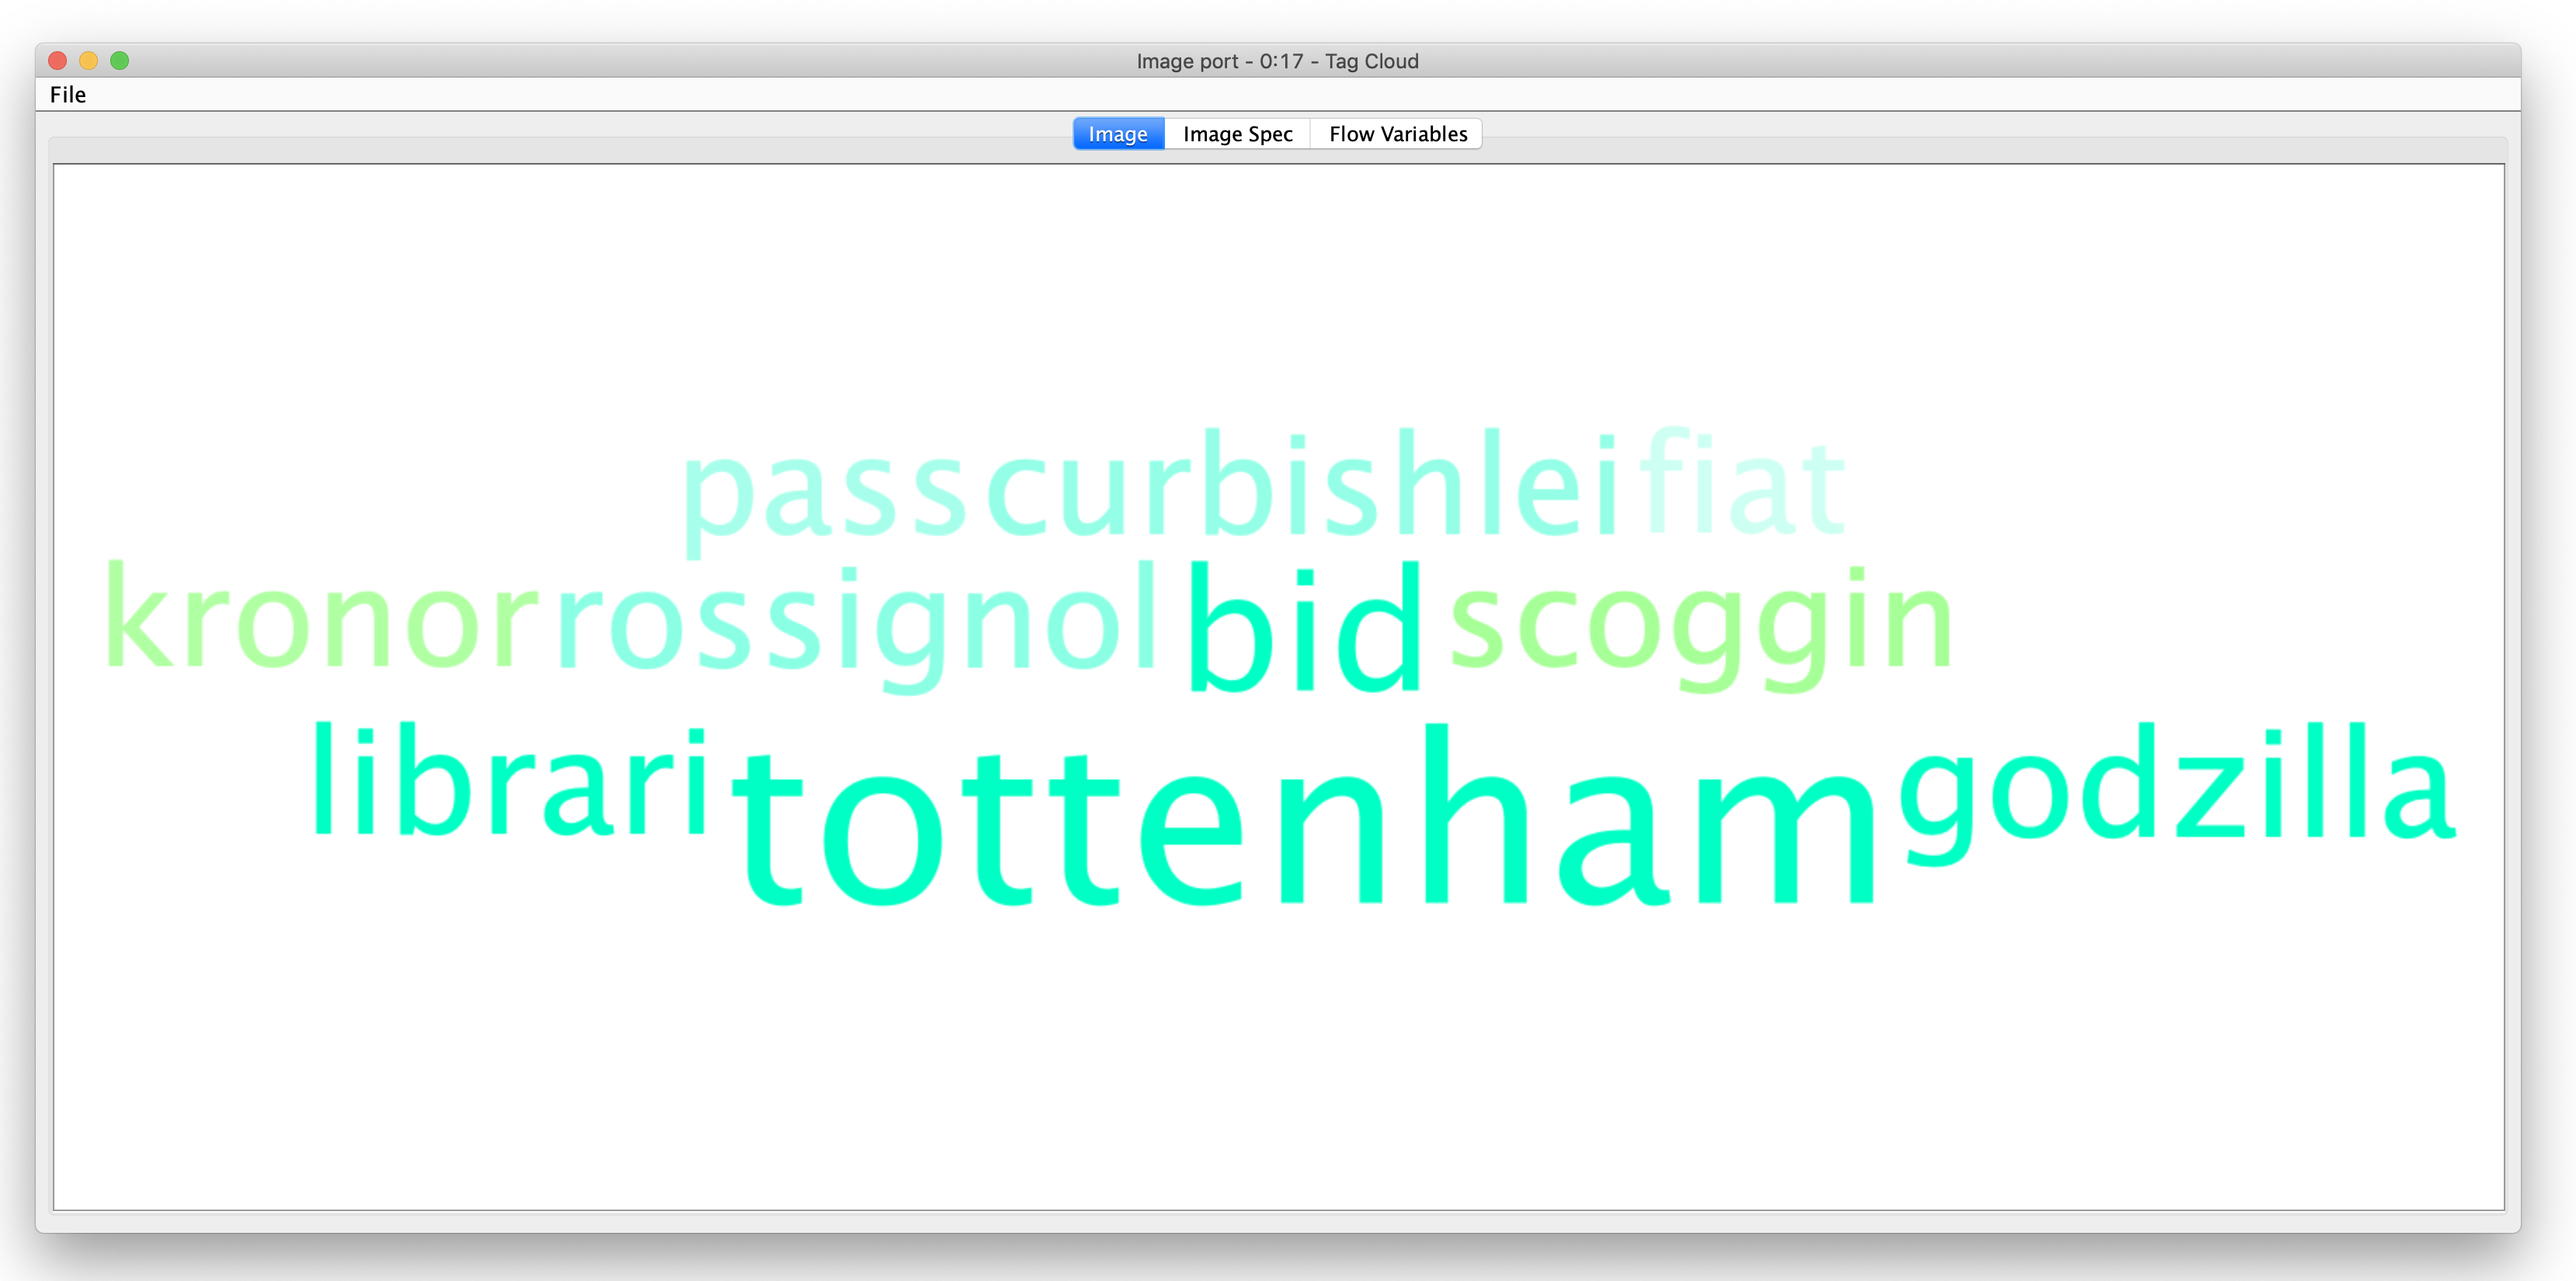
\includegraphics[width=0.9\linewidth]{images/words.png}
\end{figure}

\end{document}